% \documentclass{article}
\documentclass{standalone}
% \tikzset{
%   % style to apply some styles to each segment of a path
%   on each segment/.style={
%     decorate,
%     decoration={
%       show path construction,
%       moveto code={},
%       lineto code={
%         \path [#1]
%         (\tikzinputsegmentfirst) -- (\tikzinputsegmentlast);
%       },
%       curveto code={
%         \path [#1] (\tikzinputsegmentfirst)
%         .. controls
%         (\tikzinputsegmentsupporta) and (\tikzinputsegmentsupportb)
%         ..
%         (\tikzinputsegmentlast);
%       },
%       closepath code={
%         \path [#1]
%         (\tikzinputsegmentfirst) -- (\tikzinputsegmentlast);
%       },
%     },
%   },
%   % style to add an arrow in the middle of a path
%   mid arrow/.style={postaction={decorate,decoration={
%         markings,
%         mark=at position .5 with {\arrow[#1]{stealth}}
%       }}},
% }



\usepackage{tikz}

% \begin{tikzpicture}[very thick,decoration={
%     markings,
%     mark=at position 0.5 with {\arrow{>}}}
%     ] 
%     \draw[postaction={decorate}] (-4,0)--(4,0);
%     \draw[postaction={decorate}] (4,0)--(4,2);
%     \draw[postaction={decorate}] (4,2)--(-4,2);
%     \draw[postaction={decorate}] (-4,2)--(-4,0);
% \end{tikzpicture}

\begin{document}
    % \usetikzlibrary{decorations.markings}

  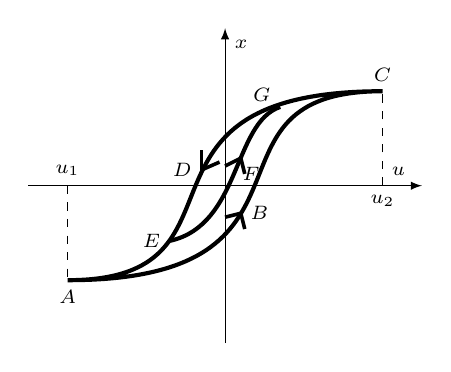
\begin{tikzpicture}
    % \draw[postaction={decorate}] (-4,0)--(4,0);
    % \draw[postaction={decorate}] (4,0)--(4,2);
    % \draw[postaction={decorate}] (4,2)--(-4,2);
    % \draw[postaction={decorate}] (-4,2)--(-4,0);
  

     \draw[line width=1.5pt] (-2,-1.2) .. controls (1.5,-1.2) and (-0.5,1.2) .. (2,1.2) .. controls (-1.5,1.2) and (0.5,-1.2) ..(-2,-1.2);

  \draw[line width=1.5pt] (-0.7,-0.7) .. controls (0.2,-0.5) and (0.1,0.8) .. (0.7, 1.);
    
    \draw[-latex] (-2.5,0) -- (2.5,0);
    \node[above] at (2.2, 0) {\scriptsize{$u$}};
    \draw[-latex] (0,-2) -- (0,2);
    \node[right] at (0, 1.8) {\scriptsize{$x$}};

    \draw[dashed] (-2,0) node[above]{\scriptsize $u_1$} -- (-2,-1.2)node[below] {\scriptsize $A$};
    \node[right] at (0.2,-0.35) {\scriptsize $B$};
    \draw[dashed] (2,0) node[below]{\scriptsize $u_2$} -- (2,1.2)node[above] {\scriptsize{$C$}};
    \node[left] at (-0.3,0.2) {\scriptsize{$D$}};
    
    \draw[line width=1.3pt] (0.2,-0.35) -- (0.25,-0.55);
    \draw[line width=1.3pt] (0.2,-0.35) -- (0,-0.40);

    \draw[line width=1.3pt] (0.2,0.35) -- (0.25,0.15);
    \draw[line width=1.3pt] (0.2,0.35) -- (0,0.25);

    \draw[line width=1.3pt] (-0.3,0.2) -- (-0.3,0.45);
     \draw[line width=1.3pt] (-0.3,0.2) -- (-0.07,0.3);    
    
    \node[left] at (-0.7,-0.7) {\scriptsize $E$};
    \node[right] at (0.1,0.15) {\scriptsize $F$};
    \node[left] at (0.7, 1.15) {\scriptsize $G$};
         

\end{tikzpicture}
\end{document}
